
% Default to the notebook output style

    


% Inherit from the specified cell style.




    
\documentclass[11pt]{article}

    
    
    \usepackage[T1]{fontenc}
    % Nicer default font (+ math font) than Computer Modern for most use cases
    \usepackage{mathpazo}

    % Basic figure setup, for now with no caption control since it's done
    % automatically by Pandoc (which extracts ![](path) syntax from Markdown).
    \usepackage{graphicx}
    % We will generate all images so they have a width \maxwidth. This means
    % that they will get their normal width if they fit onto the page, but
    % are scaled down if they would overflow the margins.
    \makeatletter
    \def\maxwidth{\ifdim\Gin@nat@width>\linewidth\linewidth
    \else\Gin@nat@width\fi}
    \makeatother
    \let\Oldincludegraphics\includegraphics
    % Set max figure width to be 80% of text width, for now hardcoded.
    \renewcommand{\includegraphics}[1]{\Oldincludegraphics[width=.8\maxwidth]{#1}}
    % Ensure that by default, figures have no caption (until we provide a
    % proper Figure object with a Caption API and a way to capture that
    % in the conversion process - todo).
    \usepackage{caption}
    \DeclareCaptionLabelFormat{nolabel}{}
    \captionsetup{labelformat=nolabel}

    \usepackage{adjustbox} % Used to constrain images to a maximum size 
    \usepackage{xcolor} % Allow colors to be defined
    \usepackage{enumerate} % Needed for markdown enumerations to work
    \usepackage{geometry} % Used to adjust the document margins
    \usepackage{amsmath} % Equations
    \usepackage{amssymb} % Equations
    \usepackage{textcomp} % defines textquotesingle
    % Hack from http://tex.stackexchange.com/a/47451/13684:
    \AtBeginDocument{%
        \def\PYZsq{\textquotesingle}% Upright quotes in Pygmentized code
    }
    \usepackage{upquote} % Upright quotes for verbatim code
    \usepackage{eurosym} % defines \euro
    \usepackage[mathletters]{ucs} % Extended unicode (utf-8) support
    \usepackage[utf8x]{inputenc} % Allow utf-8 characters in the tex document
    \usepackage{fancyvrb} % verbatim replacement that allows latex
    \usepackage{grffile} % extends the file name processing of package graphics 
                         % to support a larger range 
    % The hyperref package gives us a pdf with properly built
    % internal navigation ('pdf bookmarks' for the table of contents,
    % internal cross-reference links, web links for URLs, etc.)
    \usepackage{hyperref}
    \usepackage{longtable} % longtable support required by pandoc >1.10
    \usepackage{booktabs}  % table support for pandoc > 1.12.2
    \usepackage[inline]{enumitem} % IRkernel/repr support (it uses the enumerate* environment)
    \usepackage[normalem]{ulem} % ulem is needed to support strikethroughs (\sout)
                                % normalem makes italics be italics, not underlines
    

    
    
    % Colors for the hyperref package
    \definecolor{urlcolor}{rgb}{0,.145,.698}
    \definecolor{linkcolor}{rgb}{.71,0.21,0.01}
    \definecolor{citecolor}{rgb}{.12,.54,.11}

    % ANSI colors
    \definecolor{ansi-black}{HTML}{3E424D}
    \definecolor{ansi-black-intense}{HTML}{282C36}
    \definecolor{ansi-red}{HTML}{E75C58}
    \definecolor{ansi-red-intense}{HTML}{B22B31}
    \definecolor{ansi-green}{HTML}{00A250}
    \definecolor{ansi-green-intense}{HTML}{007427}
    \definecolor{ansi-yellow}{HTML}{DDB62B}
    \definecolor{ansi-yellow-intense}{HTML}{B27D12}
    \definecolor{ansi-blue}{HTML}{208FFB}
    \definecolor{ansi-blue-intense}{HTML}{0065CA}
    \definecolor{ansi-magenta}{HTML}{D160C4}
    \definecolor{ansi-magenta-intense}{HTML}{A03196}
    \definecolor{ansi-cyan}{HTML}{60C6C8}
    \definecolor{ansi-cyan-intense}{HTML}{258F8F}
    \definecolor{ansi-white}{HTML}{C5C1B4}
    \definecolor{ansi-white-intense}{HTML}{A1A6B2}

    % commands and environments needed by pandoc snippets
    % extracted from the output of `pandoc -s`
    \providecommand{\tightlist}{%
      \setlength{\itemsep}{0pt}\setlength{\parskip}{0pt}}
    \DefineVerbatimEnvironment{Highlighting}{Verbatim}{commandchars=\\\{\}}
    % Add ',fontsize=\small' for more characters per line
    \newenvironment{Shaded}{}{}
    \newcommand{\KeywordTok}[1]{\textcolor[rgb]{0.00,0.44,0.13}{\textbf{{#1}}}}
    \newcommand{\DataTypeTok}[1]{\textcolor[rgb]{0.56,0.13,0.00}{{#1}}}
    \newcommand{\DecValTok}[1]{\textcolor[rgb]{0.25,0.63,0.44}{{#1}}}
    \newcommand{\BaseNTok}[1]{\textcolor[rgb]{0.25,0.63,0.44}{{#1}}}
    \newcommand{\FloatTok}[1]{\textcolor[rgb]{0.25,0.63,0.44}{{#1}}}
    \newcommand{\CharTok}[1]{\textcolor[rgb]{0.25,0.44,0.63}{{#1}}}
    \newcommand{\StringTok}[1]{\textcolor[rgb]{0.25,0.44,0.63}{{#1}}}
    \newcommand{\CommentTok}[1]{\textcolor[rgb]{0.38,0.63,0.69}{\textit{{#1}}}}
    \newcommand{\OtherTok}[1]{\textcolor[rgb]{0.00,0.44,0.13}{{#1}}}
    \newcommand{\AlertTok}[1]{\textcolor[rgb]{1.00,0.00,0.00}{\textbf{{#1}}}}
    \newcommand{\FunctionTok}[1]{\textcolor[rgb]{0.02,0.16,0.49}{{#1}}}
    \newcommand{\RegionMarkerTok}[1]{{#1}}
    \newcommand{\ErrorTok}[1]{\textcolor[rgb]{1.00,0.00,0.00}{\textbf{{#1}}}}
    \newcommand{\NormalTok}[1]{{#1}}
    
    % Additional commands for more recent versions of Pandoc
    \newcommand{\ConstantTok}[1]{\textcolor[rgb]{0.53,0.00,0.00}{{#1}}}
    \newcommand{\SpecialCharTok}[1]{\textcolor[rgb]{0.25,0.44,0.63}{{#1}}}
    \newcommand{\VerbatimStringTok}[1]{\textcolor[rgb]{0.25,0.44,0.63}{{#1}}}
    \newcommand{\SpecialStringTok}[1]{\textcolor[rgb]{0.73,0.40,0.53}{{#1}}}
    \newcommand{\ImportTok}[1]{{#1}}
    \newcommand{\DocumentationTok}[1]{\textcolor[rgb]{0.73,0.13,0.13}{\textit{{#1}}}}
    \newcommand{\AnnotationTok}[1]{\textcolor[rgb]{0.38,0.63,0.69}{\textbf{\textit{{#1}}}}}
    \newcommand{\CommentVarTok}[1]{\textcolor[rgb]{0.38,0.63,0.69}{\textbf{\textit{{#1}}}}}
    \newcommand{\VariableTok}[1]{\textcolor[rgb]{0.10,0.09,0.49}{{#1}}}
    \newcommand{\ControlFlowTok}[1]{\textcolor[rgb]{0.00,0.44,0.13}{\textbf{{#1}}}}
    \newcommand{\OperatorTok}[1]{\textcolor[rgb]{0.40,0.40,0.40}{{#1}}}
    \newcommand{\BuiltInTok}[1]{{#1}}
    \newcommand{\ExtensionTok}[1]{{#1}}
    \newcommand{\PreprocessorTok}[1]{\textcolor[rgb]{0.74,0.48,0.00}{{#1}}}
    \newcommand{\AttributeTok}[1]{\textcolor[rgb]{0.49,0.56,0.16}{{#1}}}
    \newcommand{\InformationTok}[1]{\textcolor[rgb]{0.38,0.63,0.69}{\textbf{\textit{{#1}}}}}
    \newcommand{\WarningTok}[1]{\textcolor[rgb]{0.38,0.63,0.69}{\textbf{\textit{{#1}}}}}
    
    
    % Define a nice break command that doesn't care if a line doesn't already
    % exist.
    \def\br{\hspace*{\fill} \\* }
    % Math Jax compatability definitions
    \def\gt{>}
    \def\lt{<}
    % Document parameters
    \title{2.1. Syntax}
    
    
    

    % Pygments definitions
    
\makeatletter
\def\PY@reset{\let\PY@it=\relax \let\PY@bf=\relax%
    \let\PY@ul=\relax \let\PY@tc=\relax%
    \let\PY@bc=\relax \let\PY@ff=\relax}
\def\PY@tok#1{\csname PY@tok@#1\endcsname}
\def\PY@toks#1+{\ifx\relax#1\empty\else%
    \PY@tok{#1}\expandafter\PY@toks\fi}
\def\PY@do#1{\PY@bc{\PY@tc{\PY@ul{%
    \PY@it{\PY@bf{\PY@ff{#1}}}}}}}
\def\PY#1#2{\PY@reset\PY@toks#1+\relax+\PY@do{#2}}

\expandafter\def\csname PY@tok@w\endcsname{\def\PY@tc##1{\textcolor[rgb]{0.73,0.73,0.73}{##1}}}
\expandafter\def\csname PY@tok@c\endcsname{\let\PY@it=\textit\def\PY@tc##1{\textcolor[rgb]{0.25,0.50,0.50}{##1}}}
\expandafter\def\csname PY@tok@cp\endcsname{\def\PY@tc##1{\textcolor[rgb]{0.74,0.48,0.00}{##1}}}
\expandafter\def\csname PY@tok@k\endcsname{\let\PY@bf=\textbf\def\PY@tc##1{\textcolor[rgb]{0.00,0.50,0.00}{##1}}}
\expandafter\def\csname PY@tok@kp\endcsname{\def\PY@tc##1{\textcolor[rgb]{0.00,0.50,0.00}{##1}}}
\expandafter\def\csname PY@tok@kt\endcsname{\def\PY@tc##1{\textcolor[rgb]{0.69,0.00,0.25}{##1}}}
\expandafter\def\csname PY@tok@o\endcsname{\def\PY@tc##1{\textcolor[rgb]{0.40,0.40,0.40}{##1}}}
\expandafter\def\csname PY@tok@ow\endcsname{\let\PY@bf=\textbf\def\PY@tc##1{\textcolor[rgb]{0.67,0.13,1.00}{##1}}}
\expandafter\def\csname PY@tok@nb\endcsname{\def\PY@tc##1{\textcolor[rgb]{0.00,0.50,0.00}{##1}}}
\expandafter\def\csname PY@tok@nf\endcsname{\def\PY@tc##1{\textcolor[rgb]{0.00,0.00,1.00}{##1}}}
\expandafter\def\csname PY@tok@nc\endcsname{\let\PY@bf=\textbf\def\PY@tc##1{\textcolor[rgb]{0.00,0.00,1.00}{##1}}}
\expandafter\def\csname PY@tok@nn\endcsname{\let\PY@bf=\textbf\def\PY@tc##1{\textcolor[rgb]{0.00,0.00,1.00}{##1}}}
\expandafter\def\csname PY@tok@ne\endcsname{\let\PY@bf=\textbf\def\PY@tc##1{\textcolor[rgb]{0.82,0.25,0.23}{##1}}}
\expandafter\def\csname PY@tok@nv\endcsname{\def\PY@tc##1{\textcolor[rgb]{0.10,0.09,0.49}{##1}}}
\expandafter\def\csname PY@tok@no\endcsname{\def\PY@tc##1{\textcolor[rgb]{0.53,0.00,0.00}{##1}}}
\expandafter\def\csname PY@tok@nl\endcsname{\def\PY@tc##1{\textcolor[rgb]{0.63,0.63,0.00}{##1}}}
\expandafter\def\csname PY@tok@ni\endcsname{\let\PY@bf=\textbf\def\PY@tc##1{\textcolor[rgb]{0.60,0.60,0.60}{##1}}}
\expandafter\def\csname PY@tok@na\endcsname{\def\PY@tc##1{\textcolor[rgb]{0.49,0.56,0.16}{##1}}}
\expandafter\def\csname PY@tok@nt\endcsname{\let\PY@bf=\textbf\def\PY@tc##1{\textcolor[rgb]{0.00,0.50,0.00}{##1}}}
\expandafter\def\csname PY@tok@nd\endcsname{\def\PY@tc##1{\textcolor[rgb]{0.67,0.13,1.00}{##1}}}
\expandafter\def\csname PY@tok@s\endcsname{\def\PY@tc##1{\textcolor[rgb]{0.73,0.13,0.13}{##1}}}
\expandafter\def\csname PY@tok@sd\endcsname{\let\PY@it=\textit\def\PY@tc##1{\textcolor[rgb]{0.73,0.13,0.13}{##1}}}
\expandafter\def\csname PY@tok@si\endcsname{\let\PY@bf=\textbf\def\PY@tc##1{\textcolor[rgb]{0.73,0.40,0.53}{##1}}}
\expandafter\def\csname PY@tok@se\endcsname{\let\PY@bf=\textbf\def\PY@tc##1{\textcolor[rgb]{0.73,0.40,0.13}{##1}}}
\expandafter\def\csname PY@tok@sr\endcsname{\def\PY@tc##1{\textcolor[rgb]{0.73,0.40,0.53}{##1}}}
\expandafter\def\csname PY@tok@ss\endcsname{\def\PY@tc##1{\textcolor[rgb]{0.10,0.09,0.49}{##1}}}
\expandafter\def\csname PY@tok@sx\endcsname{\def\PY@tc##1{\textcolor[rgb]{0.00,0.50,0.00}{##1}}}
\expandafter\def\csname PY@tok@m\endcsname{\def\PY@tc##1{\textcolor[rgb]{0.40,0.40,0.40}{##1}}}
\expandafter\def\csname PY@tok@gh\endcsname{\let\PY@bf=\textbf\def\PY@tc##1{\textcolor[rgb]{0.00,0.00,0.50}{##1}}}
\expandafter\def\csname PY@tok@gu\endcsname{\let\PY@bf=\textbf\def\PY@tc##1{\textcolor[rgb]{0.50,0.00,0.50}{##1}}}
\expandafter\def\csname PY@tok@gd\endcsname{\def\PY@tc##1{\textcolor[rgb]{0.63,0.00,0.00}{##1}}}
\expandafter\def\csname PY@tok@gi\endcsname{\def\PY@tc##1{\textcolor[rgb]{0.00,0.63,0.00}{##1}}}
\expandafter\def\csname PY@tok@gr\endcsname{\def\PY@tc##1{\textcolor[rgb]{1.00,0.00,0.00}{##1}}}
\expandafter\def\csname PY@tok@ge\endcsname{\let\PY@it=\textit}
\expandafter\def\csname PY@tok@gs\endcsname{\let\PY@bf=\textbf}
\expandafter\def\csname PY@tok@gp\endcsname{\let\PY@bf=\textbf\def\PY@tc##1{\textcolor[rgb]{0.00,0.00,0.50}{##1}}}
\expandafter\def\csname PY@tok@go\endcsname{\def\PY@tc##1{\textcolor[rgb]{0.53,0.53,0.53}{##1}}}
\expandafter\def\csname PY@tok@gt\endcsname{\def\PY@tc##1{\textcolor[rgb]{0.00,0.27,0.87}{##1}}}
\expandafter\def\csname PY@tok@err\endcsname{\def\PY@bc##1{\setlength{\fboxsep}{0pt}\fcolorbox[rgb]{1.00,0.00,0.00}{1,1,1}{\strut ##1}}}
\expandafter\def\csname PY@tok@kc\endcsname{\let\PY@bf=\textbf\def\PY@tc##1{\textcolor[rgb]{0.00,0.50,0.00}{##1}}}
\expandafter\def\csname PY@tok@kd\endcsname{\let\PY@bf=\textbf\def\PY@tc##1{\textcolor[rgb]{0.00,0.50,0.00}{##1}}}
\expandafter\def\csname PY@tok@kn\endcsname{\let\PY@bf=\textbf\def\PY@tc##1{\textcolor[rgb]{0.00,0.50,0.00}{##1}}}
\expandafter\def\csname PY@tok@kr\endcsname{\let\PY@bf=\textbf\def\PY@tc##1{\textcolor[rgb]{0.00,0.50,0.00}{##1}}}
\expandafter\def\csname PY@tok@bp\endcsname{\def\PY@tc##1{\textcolor[rgb]{0.00,0.50,0.00}{##1}}}
\expandafter\def\csname PY@tok@fm\endcsname{\def\PY@tc##1{\textcolor[rgb]{0.00,0.00,1.00}{##1}}}
\expandafter\def\csname PY@tok@vc\endcsname{\def\PY@tc##1{\textcolor[rgb]{0.10,0.09,0.49}{##1}}}
\expandafter\def\csname PY@tok@vg\endcsname{\def\PY@tc##1{\textcolor[rgb]{0.10,0.09,0.49}{##1}}}
\expandafter\def\csname PY@tok@vi\endcsname{\def\PY@tc##1{\textcolor[rgb]{0.10,0.09,0.49}{##1}}}
\expandafter\def\csname PY@tok@vm\endcsname{\def\PY@tc##1{\textcolor[rgb]{0.10,0.09,0.49}{##1}}}
\expandafter\def\csname PY@tok@sa\endcsname{\def\PY@tc##1{\textcolor[rgb]{0.73,0.13,0.13}{##1}}}
\expandafter\def\csname PY@tok@sb\endcsname{\def\PY@tc##1{\textcolor[rgb]{0.73,0.13,0.13}{##1}}}
\expandafter\def\csname PY@tok@sc\endcsname{\def\PY@tc##1{\textcolor[rgb]{0.73,0.13,0.13}{##1}}}
\expandafter\def\csname PY@tok@dl\endcsname{\def\PY@tc##1{\textcolor[rgb]{0.73,0.13,0.13}{##1}}}
\expandafter\def\csname PY@tok@s2\endcsname{\def\PY@tc##1{\textcolor[rgb]{0.73,0.13,0.13}{##1}}}
\expandafter\def\csname PY@tok@sh\endcsname{\def\PY@tc##1{\textcolor[rgb]{0.73,0.13,0.13}{##1}}}
\expandafter\def\csname PY@tok@s1\endcsname{\def\PY@tc##1{\textcolor[rgb]{0.73,0.13,0.13}{##1}}}
\expandafter\def\csname PY@tok@mb\endcsname{\def\PY@tc##1{\textcolor[rgb]{0.40,0.40,0.40}{##1}}}
\expandafter\def\csname PY@tok@mf\endcsname{\def\PY@tc##1{\textcolor[rgb]{0.40,0.40,0.40}{##1}}}
\expandafter\def\csname PY@tok@mh\endcsname{\def\PY@tc##1{\textcolor[rgb]{0.40,0.40,0.40}{##1}}}
\expandafter\def\csname PY@tok@mi\endcsname{\def\PY@tc##1{\textcolor[rgb]{0.40,0.40,0.40}{##1}}}
\expandafter\def\csname PY@tok@il\endcsname{\def\PY@tc##1{\textcolor[rgb]{0.40,0.40,0.40}{##1}}}
\expandafter\def\csname PY@tok@mo\endcsname{\def\PY@tc##1{\textcolor[rgb]{0.40,0.40,0.40}{##1}}}
\expandafter\def\csname PY@tok@ch\endcsname{\let\PY@it=\textit\def\PY@tc##1{\textcolor[rgb]{0.25,0.50,0.50}{##1}}}
\expandafter\def\csname PY@tok@cm\endcsname{\let\PY@it=\textit\def\PY@tc##1{\textcolor[rgb]{0.25,0.50,0.50}{##1}}}
\expandafter\def\csname PY@tok@cpf\endcsname{\let\PY@it=\textit\def\PY@tc##1{\textcolor[rgb]{0.25,0.50,0.50}{##1}}}
\expandafter\def\csname PY@tok@c1\endcsname{\let\PY@it=\textit\def\PY@tc##1{\textcolor[rgb]{0.25,0.50,0.50}{##1}}}
\expandafter\def\csname PY@tok@cs\endcsname{\let\PY@it=\textit\def\PY@tc##1{\textcolor[rgb]{0.25,0.50,0.50}{##1}}}

\def\PYZbs{\char`\\}
\def\PYZus{\char`\_}
\def\PYZob{\char`\{}
\def\PYZcb{\char`\}}
\def\PYZca{\char`\^}
\def\PYZam{\char`\&}
\def\PYZlt{\char`\<}
\def\PYZgt{\char`\>}
\def\PYZsh{\char`\#}
\def\PYZpc{\char`\%}
\def\PYZdl{\char`\$}
\def\PYZhy{\char`\-}
\def\PYZsq{\char`\'}
\def\PYZdq{\char`\"}
\def\PYZti{\char`\~}
% for compatibility with earlier versions
\def\PYZat{@}
\def\PYZlb{[}
\def\PYZrb{]}
\makeatother


    % Exact colors from NB
    \definecolor{incolor}{rgb}{0.0, 0.0, 0.5}
    \definecolor{outcolor}{rgb}{0.545, 0.0, 0.0}



    
    % Prevent overflowing lines due to hard-to-break entities
    \sloppy 
    % Setup hyperref package
    \hypersetup{
      breaklinks=true,  % so long urls are correctly broken across lines
      colorlinks=true,
      urlcolor=urlcolor,
      linkcolor=linkcolor,
      citecolor=citecolor,
      }
    % Slightly bigger margins than the latex defaults
    
    \geometry{verbose,tmargin=1in,bmargin=1in,lmargin=1in,rmargin=1in}
    
    

    \begin{document}
    
    
    \maketitle
    
    

    
    \hypertarget{chapter-2-syntax-and-style-guidlines}{%
\section{Chapter 2: Syntax and Style
Guidlines}\label{chapter-2-syntax-and-style-guidlines}}

\begin{center}\rule{0.5\linewidth}{\linethickness}\end{center}

    \begin{quote}
\textbf{code is read much more often than it is written} -- Guido's key
insights
\end{quote}

One of the main feature of Python is that it forces the developers to
write the code with proper formatting. Failing to do so will
\textbf{always} result in invalid code. It has been achived by removing
the need for block markers, such as curly brackets ``\{ \}'' which are
so commonly used in most of the languages such as C/C++ \& Java. It
instead use spaces/tab.

In this section we will be discussing major points of language syntax
such as comments, blocks multiline code and introduction to PEP 8

    The command \texttt{print} inserts spaces between expressions that are
received as a parameter, and a newline character at the end, unless it
receives a comma at the end of the parameter list.

\hypertarget{blocks}{%
\subsection{Blocks}\label{blocks}}

In Python, code blocks are defined by the use of indentation, which
should be constant in the code block, but it is considered good practice
to maintain consistency throughout the project and avoid mixing tabs and
{spaces}.

The line before the block always ends with a colon (:) and is a control
structure of the language or a statement of a new structure (function,
class for example).

\begin{figure}
\centering
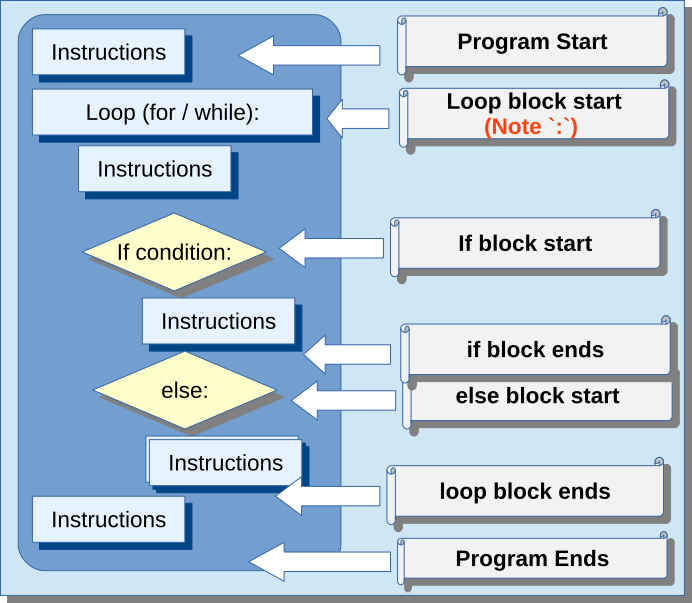
\includegraphics{files/blocks.png}
\caption{Program structure}
\end{figure}

    \hypertarget{code-layout}{%
\subsection{\#\# Code layout}\label{code-layout}}

\hypertarget{lines-and-indentation}{%
\subsection{\#\#\# Lines and Indentation}\label{lines-and-indentation}}

Python don't use braces \texttt{\{\}}, as most programming languages
use, to mark blocks of code for classes, function definitions and flow
controls. Blocks of code are denoted by line indentation, which is
rigidly enforced.

The number of spaces in the indentation should be same to mark the
block, such as if 4 spaces or 1 tab is used, then it should be
consistent for entire project or in other words, all statements within
the block must be indented by the same amount of space or tab.

\emph{Example}:

    \begin{Verbatim}[commandchars=\\\{\}]
{\color{incolor}In [{\color{incolor}1}]:} \PY{k}{if} \PY{k+kc}{True}\PY{p}{:}
            \PY{n+nb}{print}\PY{p}{(}\PY{l+s+s2}{\PYZdq{}}\PY{l+s+s2}{True}\PY{l+s+s2}{\PYZdq{}}\PY{p}{)}
        \PY{k}{else}\PY{p}{:}
            \PY{n+nb}{print}\PY{p}{(}\PY{l+s+s2}{\PYZdq{}}\PY{l+s+s2}{False}\PY{l+s+s2}{\PYZdq{}}\PY{p}{)}
\end{Verbatim}


    \begin{Verbatim}[commandchars=\\\{\}]
True

    \end{Verbatim}

    \begin{Verbatim}[commandchars=\\\{\}]
{\color{incolor}In [{\color{incolor}2}]:} \PY{k}{if} \PY{k+kc}{True}\PY{p}{:}
                    \PY{n+nb}{print}\PY{p}{(}\PY{l+s+s2}{\PYZdq{}}\PY{l+s+s2}{True}\PY{l+s+s2}{\PYZdq{}}\PY{p}{)}
        \PY{k}{else}\PY{p}{:}
                    \PY{n+nb}{print}\PY{p}{(}\PY{l+s+s2}{\PYZdq{}}\PY{l+s+s2}{False}\PY{l+s+s2}{\PYZdq{}}\PY{p}{)}
\end{Verbatim}


    \begin{Verbatim}[commandchars=\\\{\}]
True

    \end{Verbatim}

    \begin{Verbatim}[commandchars=\\\{\}]
{\color{incolor}In [{\color{incolor}3}]:} \PY{k}{if} \PY{p}{(}\PY{k+kc}{True}\PY{p}{)}\PY{p}{:}  
            \PY{n+nb}{print}\PY{p}{(}\PY{l+s+s2}{\PYZdq{}}\PY{l+s+s2}{True}\PY{l+s+s2}{\PYZdq{}}\PY{p}{)} 
        \PY{k}{else}\PY{p}{:}  
            \PY{n+nb}{print}\PY{p}{(}\PY{l+s+s2}{\PYZdq{}}\PY{l+s+s2}{Test}\PY{l+s+s2}{\PYZdq{}}\PY{p}{)}
               \PY{n+nb}{print}\PY{p}{(}\PY{l+s+s2}{\PYZdq{}}\PY{l+s+s2}{False}\PY{l+s+s2}{\PYZdq{}}\PY{p}{)}
\end{Verbatim}


    \begin{Verbatim}[commandchars=\\\{\}]

          File "<ipython-input-3-155005a566f3>", line 5
        print("False")
        \^{}
    IndentationError: unexpected indent
    

    \end{Verbatim}

    Execution of below block of code will result in \texttt{error} as the
indentation level is not uniform.

    \begin{Verbatim}[commandchars=\\\{\}]
{\color{incolor}In [{\color{incolor}2}]:} \PY{k}{if} \PY{k+kc}{True}\PY{p}{:}
            \PY{n+nb}{print}\PY{p}{(}\PY{l+s+s2}{\PYZdq{}}\PY{l+s+s2}{Answer}\PY{l+s+s2}{\PYZdq{}}\PY{p}{)}
            \PY{n+nb}{print}\PY{p}{(}\PY{l+s+s2}{\PYZdq{}}\PY{l+s+s2}{True}\PY{l+s+s2}{\PYZdq{}}\PY{p}{)}
        \PY{k}{else}\PY{p}{:}
            \PY{n+nb}{print}\PY{p}{(}\PY{l+s+s2}{\PYZdq{}}\PY{l+s+s2}{Answer}\PY{l+s+s2}{\PYZdq{}}\PY{p}{)}
             \PY{n+nb}{print}\PY{p}{(}\PY{l+s+s2}{\PYZdq{}}\PY{l+s+s2}{False}\PY{l+s+s2}{\PYZdq{}}\PY{p}{)}
\end{Verbatim}


    \begin{Verbatim}[commandchars=\\\{\}]

          File "<ipython-input-2-37066c257527>", line 6
        print("False")
        \^{}
    IndentationError: unexpected indent
    

    \end{Verbatim}

    \begin{Verbatim}[commandchars=\\\{\}]
{\color{incolor}In [{\color{incolor}5}]:} \PY{k}{if} \PY{k+kc}{True}\PY{p}{:} \PY{c+c1}{\PYZsh{}\PYZob{}}
            \PY{n+nb}{print}\PY{p}{(}\PY{l+s+s2}{\PYZdq{}}\PY{l+s+s2}{Answer}\PY{l+s+s2}{\PYZdq{}}\PY{p}{)}
            \PY{n+nb}{print}\PY{p}{(}\PY{l+s+s2}{\PYZdq{}}\PY{l+s+s2}{True}\PY{l+s+s2}{\PYZdq{}}\PY{p}{)}
            \PY{c+c1}{\PYZsh{}\PYZcb{}}
        \PY{k}{else}\PY{p}{:} \PY{c+c1}{\PYZsh{}\PYZob{}}
            \PY{n+nb}{print}\PY{p}{(}\PY{l+s+s2}{\PYZdq{}}\PY{l+s+s2}{Answer}\PY{l+s+s2}{\PYZdq{}}\PY{p}{)}
            \PY{n+nb}{print}\PY{p}{(}\PY{l+s+s2}{\PYZdq{}}\PY{l+s+s2}{False}\PY{l+s+s2}{\PYZdq{}}\PY{p}{)}
            \PY{c+c1}{\PYZsh{}\PYZcb{}}
\end{Verbatim}


    \begin{Verbatim}[commandchars=\\\{\}]
Answer
True

    \end{Verbatim}

    The closing brace/bracket/parenthesis on multi-line constructs may
either line up under the first non-whitespace character of the last line
of list, as in:

    \begin{Verbatim}[commandchars=\\\{\}]
{\color{incolor}In [{\color{incolor}7}]:} \PY{k}{def} \PY{n+nf}{func}\PY{p}{(}\PY{n}{x}\PY{p}{,}\PY{n}{y}\PY{p}{,}\PY{n}{z}\PY{p}{,}\PY{n}{m}\PY{p}{,}\PY{n}{n}\PY{p}{,}\PY{n}{r}\PY{p}{)}\PY{p}{:}
            \PY{n+nb}{print}\PY{p}{(}\PY{n}{x}\PY{p}{,}\PY{n}{y}\PY{p}{,}\PY{n}{z}\PY{p}{,}\PY{n}{m}\PY{p}{,}\PY{n}{n}\PY{p}{,}\PY{n}{r}\PY{p}{)}
        
        \PY{n}{my\PYZus{}list} \PY{o}{=} \PY{p}{[}
            \PY{l+m+mi}{1}\PY{p}{,} \PY{l+m+mi}{2}\PY{p}{,} \PY{l+m+mi}{3}\PY{p}{,}
            \PY{l+m+mi}{4}\PY{p}{,} \PY{l+m+mi}{5}\PY{p}{,} \PY{l+m+mi}{6}
            \PY{p}{]}
        \PY{n}{result} \PY{o}{=} \PY{n}{func}\PY{p}{(}
            \PY{l+s+s1}{\PYZsq{}}\PY{l+s+s1}{a}\PY{l+s+s1}{\PYZsq{}}\PY{p}{,} \PY{l+s+s1}{\PYZsq{}}\PY{l+s+s1}{b}\PY{l+s+s1}{\PYZsq{}}\PY{p}{,} \PY{l+s+s1}{\PYZsq{}}\PY{l+s+s1}{c}\PY{l+s+s1}{\PYZsq{}}\PY{p}{,}
            \PY{l+s+s1}{\PYZsq{}}\PY{l+s+s1}{d}\PY{l+s+s1}{\PYZsq{}}\PY{p}{,} \PY{l+s+s1}{\PYZsq{}}\PY{l+s+s1}{e}\PY{l+s+s1}{\PYZsq{}}\PY{p}{,} \PY{l+s+s1}{\PYZsq{}}\PY{l+s+s1}{f}\PY{l+s+s1}{\PYZsq{}}
            \PY{p}{)}
\end{Verbatim}


    \begin{Verbatim}[commandchars=\\\{\}]
a b c d e f

    \end{Verbatim}

    or it may be lined up under the first character of the line that starts
the multi-line construct, as in:

    \begin{Verbatim}[commandchars=\\\{\}]
{\color{incolor}In [{\color{incolor}9}]:} \PY{k}{def} \PY{n+nf}{some\PYZus{}function\PYZus{}that\PYZus{}takes\PYZus{}arguments}\PY{p}{(}\PY{n}{a1}\PY{p}{,}\PY{n}{a2}\PY{p}{,}\PY{n}{a3}\PY{p}{,}\PY{n}{a4}\PY{p}{,}\PY{n}{a5}\PY{p}{,}\PY{n}{a6}\PY{p}{)}\PY{p}{:}
            \PY{k}{pass}
        
        \PY{n}{my\PYZus{}list} \PY{o}{=} \PY{p}{[}
            \PY{l+m+mi}{1}\PY{p}{,} \PY{l+m+mi}{2}\PY{p}{,} \PY{l+m+mi}{3}\PY{p}{,}
            \PY{l+m+mi}{4}\PY{p}{,} \PY{l+m+mi}{5}\PY{p}{,} \PY{l+m+mi}{6}\PY{p}{,}
        \PY{p}{]}
        \PY{n}{result} \PY{o}{=} \PY{n}{some\PYZus{}function\PYZus{}that\PYZus{}takes\PYZus{}arguments}\PY{p}{(}
            \PY{l+s+s1}{\PYZsq{}}\PY{l+s+s1}{a}\PY{l+s+s1}{\PYZsq{}}\PY{p}{,} \PY{l+s+s1}{\PYZsq{}}\PY{l+s+s1}{b}\PY{l+s+s1}{\PYZsq{}}\PY{p}{,} \PY{l+s+s1}{\PYZsq{}}\PY{l+s+s1}{c}\PY{l+s+s1}{\PYZsq{}}\PY{p}{,}
            \PY{l+s+s1}{\PYZsq{}}\PY{l+s+s1}{d}\PY{l+s+s1}{\PYZsq{}}\PY{p}{,} \PY{l+s+s1}{\PYZsq{}}\PY{l+s+s1}{e}\PY{l+s+s1}{\PYZsq{}}\PY{p}{,} \PY{l+s+s1}{\PYZsq{}}\PY{l+s+s1}{f}\PY{l+s+s1}{\PYZsq{}}
        \PY{p}{)}
\end{Verbatim}


    \hypertarget{comments}{%
\subsection{\#\# Comments}\label{comments}}

The character \texttt{\#} marks the beginning of a comment. Any text
after the \texttt{\#} will be ignored until the end of the line, with
the exception of functional comments.

Functional comments are used to:

\begin{itemize}
\tightlist
\item
  change the encoding of the source file of the program by adding a
  comment with the text
  \texttt{\#\ -\ *\ -\ coding:\ \ \textless{}encoding\textgreater{}\ -\ \#\ -}
  at the beginning of the file, in which
  \texttt{\textless{}encoding\textgreater{}} is the file encoding
  (usually latin1 or utf-8). Changing encoding is required to support
  characters that are not part of the English language, in the source
  code of the program.
\item
  define the interpreter that will be used to run the program on UNIX
  systems, through a comment starting with \texttt{\#!} at the beginning
  of the file, which indicates the path to the interpreter (usually the
  comment line will be something like \texttt{\#!/usr/bin/env\ python}
  ).
\end{itemize}

    \hypertarget{block-comments}{%
\subsection{\#\# Block Comments}\label{block-comments}}

Block comments generally apply to some (or all) code that follows them,
and are indented to the same level as that code. Each line of a block
comment starts with a \# and a single space (unless it is indented text
inside the comment).

Paragraphs inside a block comment are separated by a line containing a
single \# .

\begin{Shaded}
\begin{Highlighting}[]
\CommentTok{# Date: }
\CommentTok{# Time:}
\CommentTok{# Author:}
\CommentTok{# Method Name:}
\CommentTok{# Description: }
\end{Highlighting}
\end{Shaded}

\hypertarget{inline-comments}{%
\subsection{\#\# Inline Comments}\label{inline-comments}}

Use inline comments sparingly.

An inline comment is a comment on the same line as a statement. Inline
comments should be separated by at least two spaces from the statement.
They should start with a \# and a single space.

Inline comments are unnecessary and in fact distracting if they state
the obvious. Don't do this:

\begin{Shaded}
\begin{Highlighting}[]
\NormalTok{x }\OperatorTok{=}\NormalTok{ x }\OperatorTok{+} \DecValTok{1}                 \CommentTok{# Increment x}
\end{Highlighting}
\end{Shaded}

But sometimes, it is useful as shown below:

\begin{Shaded}
\begin{Highlighting}[]
\NormalTok{x }\OperatorTok{=}\NormalTok{ x }\OperatorTok{+} \DecValTok{1}                 \CommentTok{# Compensate for border}
\end{Highlighting}
\end{Shaded}

    \hypertarget{tips-for-comments}{%
\subsection{\#\# Tips for Comments}\label{tips-for-comments}}

\begin{itemize}
\tightlist
\item
  Comments that contradict the code are worse than no comments. Always
  make a priority of keeping the comments up-to-date when the code
  changes!
\item
  Comments should be complete sentences. If a comment is a phrase or
  sentence, its first word should be capitalized, unless it is an
  identifier that begins with a lower case letter (never alter the case
  of identifiers!).
\item
  If a comment is short, the period at the end can be omitted. Block
  comments generally consist of one or more paragraphs built out of
  complete sentences, and each sentence should end in a period.
\item
  You should use two spaces after a sentence-ending period.
\item
  When writing English, follow Strunk and White.
\item
  Python coders from non-English speaking countries: please write your
  comments in English, unless you are 120\% sure that the code will
  never be read by people who don't speak your language.
\end{itemize}

    \begin{Verbatim}[commandchars=\\\{\}]
{\color{incolor}In [{\color{incolor}6}]:} \PY{c+ch}{\PYZsh{}!/usr/bin/env python}
        
        \PY{c+c1}{\PYZsh{} A code line that shows the result of 7 times 3}
        \PY{c+c1}{\PYZsh{} A CODE LINE THAT SHOW THE RESULT OF 7 TIMES 3 (BAD Comments)}
        
        \PY{n+nb}{print} \PY{p}{(}\PY{l+m+mi}{7} \PY{o}{*} \PY{l+m+mi}{3}\PY{p}{)} \PY{c+c1}{\PYZsh{} This is also a comment}
        \PY{l+s+sd}{\PYZdq{}\PYZdq{}\PYZdq{}}
        \PY{l+s+sd}{This is a multi}
        \PY{l+s+sd}{line comment / String}
        \PY{l+s+sd}{\PYZdq{}\PYZdq{}\PYZdq{}}
        \PY{n}{st} \PY{o}{=} \PY{l+s+s1}{\PYZsq{}\PYZsq{}\PYZsq{}}
        \PY{l+s+s1}{This is a multi line }
        
        \PY{l+s+s1}{String}
        \PY{l+s+s1}{\PYZdq{}}\PY{l+s+s1}{With me}\PY{l+s+s1}{\PYZdq{}}
        \PY{l+s+s1}{\PYZsq{}}
        \PY{l+s+s1}{\PYZsq{}}
        \PY{l+s+s1}{\PYZsq{}\PYZsq{}\PYZsq{}}
        \PY{n+nb}{print}\PY{p}{(}\PY{n}{st}\PY{p}{)}
\end{Verbatim}


    \begin{Verbatim}[commandchars=\\\{\}]
21

This is a multi line 

String
"With me"
'
'


    \end{Verbatim}

    \hypertarget{indentation}{%
\subsection{\#\#\# Indentation}\label{indentation}}

\begin{itemize}
\tightlist
\item
  Use 4 spaces per indentation level
\item
  If your code has continuation lines, then they should align wrapped
  elements either vertically using Python''s implicit line joining
  inside parentheses, brackets and braces, or using a \textbf{hanging
  indent}.
\item
  When using a hanging indent the following should be considered; there
  should be no arguments on the first line and further indentation
  should be used to clearly distinguish itself as a continuation line.
\end{itemize}

    \begin{Verbatim}[commandchars=\\\{\}]
{\color{incolor}In [{\color{incolor} }]:} \PY{c+c1}{\PYZsh{} More indentation included to distinguish this from the rest.}
        \PY{k}{def} \PY{n+nf}{long\PYZus{}function\PYZus{}name}\PY{p}{(}
                \PY{n}{var\PYZus{}one}\PY{p}{,} \PY{n}{var\PYZus{}two}\PY{p}{,} \PY{n}{var\PYZus{}three}\PY{p}{,}
                \PY{n}{var\PYZus{}four}\PY{p}{)}\PY{p}{:}
            \PY{n+nb}{print}\PY{p}{(}\PY{n}{var\PYZus{}one}\PY{p}{)}
            
        \PY{c+c1}{\PYZsh{} Aligned with opening delimiter.}
        \PY{n}{foo} \PY{o}{=} \PY{n}{long\PYZus{}function\PYZus{}name}\PY{p}{(}\PY{l+s+s2}{\PYZdq{}}\PY{l+s+s2}{var\PYZus{}one}\PY{l+s+s2}{\PYZdq{}}\PY{p}{,} \PY{l+s+s2}{\PYZdq{}}\PY{l+s+s2}{var\PYZus{}two}\PY{l+s+s2}{\PYZdq{}}\PY{p}{,}
                                 \PY{l+s+s2}{\PYZdq{}}\PY{l+s+s2}{var\PYZus{}three}\PY{l+s+s2}{\PYZdq{}}\PY{p}{,} \PY{l+s+s2}{\PYZdq{}}\PY{l+s+s2}{var\PYZus{}four}\PY{l+s+s2}{\PYZdq{}}\PY{p}{)}
        
        
        \PY{c+c1}{\PYZsh{} Hanging indents should add a level.}
        \PY{n}{foo} \PY{o}{=} \PY{n}{long\PYZus{}function\PYZus{}name}\PY{p}{(}
            \PY{l+s+s2}{\PYZdq{}}\PY{l+s+s2}{var\PYZus{}one}\PY{l+s+s2}{\PYZdq{}}\PY{p}{,} \PY{l+s+s2}{\PYZdq{}}\PY{l+s+s2}{var\PYZus{}two}\PY{l+s+s2}{\PYZdq{}}\PY{p}{,}
            \PY{l+s+s2}{\PYZdq{}}\PY{l+s+s2}{var\PYZus{}three}\PY{l+s+s2}{\PYZdq{}}\PY{p}{,} \PY{l+s+s2}{\PYZdq{}}\PY{l+s+s2}{var\PYZus{}four}\PY{l+s+s2}{\PYZdq{}}\PY{p}{)}
\end{Verbatim}


    \hypertarget{tabs-or-spaces}{%
\subsection{\#\# Tabs or Spaces?}\label{tabs-or-spaces}}

\begin{quote}
\textbf{``''``'' Spaces are the preferred indentation method ``''``''}
\end{quote}

Tabs should be used solely to remain consistent with code that is
already indented with tabs.

\begin{quote}
Python 3 disallows mixing the use of tabs and spaces for indentation.
\end{quote}

    \hypertarget{maximum-line-length}{%
\subsection{\#\#\# Maximum Line Length}\label{maximum-line-length}}

\begin{itemize}
\item
  Limit all lines to a maximum of 79 characters.
\item
  For flowing long blocks of text with fewer structural restrictions
  (docstrings or comments), the line length should be limited to 72
  characters.
\item
  Limiting the required editor window width makes it possible to have
  several files open side-by-side, and works well when using code review
  tools that present the two versions in adjacent columns.
\item
  The default wrapping in most tools disrupts the visual structure of
  the code, making it more difficult to understand. The limits are
  chosen to avoid wrapping in editors with the window width set to 80,
  even if the tool places a marker glyph in the final column when
  wrapping lines. Some web based tools may not offer dynamic line
  wrapping at all.
\item
  Some teams strongly prefer a longer line length. For code maintained
  exclusively or primarily by a team that can reach agreement on this
  issue, it is okay to increase the nominal line length from 80 to 100
  characters (effectively increasing the maximum length to 99
  characters), provided that comments and docstrings are still wrapped
  at 72 characters.
\item
  The Python standard library is conservative and requires limiting
  lines to 79 characters (and docstrings/comments to 72).
\item
  The preferred way of wrapping long lines is by using Python's implied
  line continuation inside parentheses, brackets and braces. Long lines
  can be broken over multiple lines by wrapping expressions in
  parentheses. These should be used in preference to using a backslash
  for line continuation.
\item
  Backslashes may still be appropriate at times. For example, long,
  multiple with -statements cannot use implicit continuation, so
  backslashes are acceptable:
\end{itemize}

    \begin{Verbatim}[commandchars=\\\{\}]
{\color{incolor}In [{\color{incolor} }]:} \PY{k}{with} \PY{n+nb}{open}\PY{p}{(}\PY{l+s+s1}{\PYZsq{}}\PY{l+s+s1}{/path/to/some/file/you/want/to/read}\PY{l+s+s1}{\PYZsq{}}\PY{p}{)} \PY{k}{as} \PY{n}{file\PYZus{}1}\PY{p}{,} \PYZbs{}
             \PY{n+nb}{open}\PY{p}{(}\PY{l+s+s1}{\PYZsq{}}\PY{l+s+s1}{/path/to/some/file/being/written}\PY{l+s+s1}{\PYZsq{}}\PY{p}{,} \PY{l+s+s1}{\PYZsq{}}\PY{l+s+s1}{w}\PY{l+s+s1}{\PYZsq{}}\PY{p}{)} \PY{k}{as} \PY{n}{file\PYZus{}2}\PY{p}{:}
            \PY{n}{file\PYZus{}2}\PY{o}{.}\PY{n}{write}\PY{p}{(}\PY{n}{file\PYZus{}1}\PY{o}{.}\PY{n}{read}\PY{p}{(}\PY{p}{)}\PY{p}{)}
\end{Verbatim}


    \hypertarget{multiline-code}{%
\subsection{\#\# Multiline code}\label{multiline-code}}

In Python, multi-line code is supported by using the backslash character
(\texttt{\textbackslash{}}) at the end of the line or parentheses,
brackets or braces in expressions that use such characters.

Examples of broken lines:

    \begin{Verbatim}[commandchars=\\\{\}]
{\color{incolor}In [{\color{incolor}10}]:} \PY{c+c1}{\PYZsh{} A line broken by backslash}
         \PY{n}{a} \PY{o}{=} \PY{l+m+mi}{7} \PY{o}{*} \PY{l+m+mi}{3} \PY{o}{+} \PYZbs{}
         \PY{l+m+mi}{5} \PY{o}{/} \PY{l+m+mi}{2}
         
         
         \PY{c+c1}{\PYZsh{} A list (broken by comma)}
         \PY{n}{b} \PY{o}{=} \PY{p}{[}\PY{l+s+s1}{\PYZsq{}}\PY{l+s+s1}{a}\PY{l+s+s1}{\PYZsq{}}\PY{p}{,} \PY{l+s+s1}{\PYZsq{}}\PY{l+s+s1}{b}\PY{l+s+s1}{\PYZsq{}}\PY{p}{,} \PY{l+s+s1}{\PYZsq{}}\PY{l+s+s1}{c}\PY{l+s+s1}{\PYZsq{}}\PY{p}{,} 
         \PY{l+s+s1}{\PYZsq{}}\PY{l+s+s1}{d}\PY{l+s+s1}{\PYZsq{}}\PY{p}{,} \PY{l+s+s1}{\PYZsq{}}\PY{l+s+s1}{e}\PY{l+s+s1}{\PYZsq{}}\PY{p}{]}
         
         \PY{c+c1}{\PYZsh{} A function call (broken by comma)}
         \PY{n}{c} \PY{o}{=} \PY{n+nb}{range}\PY{p}{(}\PY{l+m+mi}{1}\PY{p}{,}
                 \PY{l+m+mi}{11}\PY{p}{)}
         
         \PY{c+c1}{\PYZsh{} Prints everything}
         \PY{n+nb}{print}\PY{p}{(}\PY{n}{a}\PY{p}{,} \PY{n}{b}\PY{p}{,} \PY{n}{c}\PY{p}{)}
\end{Verbatim}


    \begin{Verbatim}[commandchars=\\\{\}]
23.5 ['a', 'b', 'c', 'd', 'e'] range(1, 11)

    \end{Verbatim}

    \begin{Verbatim}[commandchars=\\\{\}]
{\color{incolor}In [{\color{incolor}14}]:} \PY{c+c1}{\PYZsh{} For i on the list 234, 654, 378, 798:}
         \PY{k}{for} \PY{n}{i} \PY{o+ow}{in} \PY{p}{[}\PY{l+m+mi}{234}\PY{p}{,} \PY{l+m+mi}{654}\PY{p}{,} \PY{l+m+mi}{378}\PY{p}{,} \PY{l+m+mi}{798}\PY{p}{]}\PY{p}{:}
             \PY{c+c1}{\PYZsh{} If the remainder dividing by 3 is equal to zero:}
             \PY{k}{if} \PY{n}{i} \PY{o}{\PYZpc{}} \PY{l+m+mi}{3} \PY{o}{==} \PY{l+m+mi}{0}\PY{p}{:} \PY{c+c1}{\PYZsh{}\PYZob{}}
                \PY{c+c1}{\PYZsh{} Prints...}
                 \PY{n+nb}{print} \PY{p}{(}\PY{n}{i}\PY{p}{,} \PY{l+s+s1}{\PYZsq{}}\PY{l+s+s1}{/ 3 =}\PY{l+s+s1}{\PYZsq{}}\PY{p}{,} \PY{n}{i} \PY{o}{/} \PY{l+m+mi}{3}\PY{p}{)}
             \PY{c+c1}{\PYZsh{}\PYZcb{}}
\end{Verbatim}


    \begin{Verbatim}[commandchars=\\\{\}]
234 / 3 = 78.0
654 / 3 = 218.0
378 / 3 = 126.0
798 / 3 = 266.0

    \end{Verbatim}

    The operator \texttt{\%} computes the modulus (remainder of division).

    \hypertarget{line-break-before-or-after-a-binary-operator}{%
\subsection{\#\#\# line break before or after a binary
operator}\label{line-break-before-or-after-a-binary-operator}}

Donald Knuth explains the traditional rule in his Computers and
Typesetting series: ``Although formulas within a paragraph always break
after binary operations and relations, displayed formulas always break
before binary operations''.

Following the tradition from mathematics usually results in more
readable code:

    \begin{Verbatim}[commandchars=\\\{\}]
{\color{incolor}In [{\color{incolor}2}]:} \PY{c+c1}{\PYZsh{} Yes: easy to match operators with operands}
        \PY{n}{income} \PY{o}{=} \PY{p}{(}\PY{n}{gross\PYZus{}wages}
                  \PY{o}{+} \PY{n}{taxable\PYZus{}interest}
                  \PY{o}{+} \PY{p}{(}\PY{n}{dividends} \PY{o}{\PYZhy{}} \PY{n}{qualified\PYZus{}dividends}\PY{p}{)}
                  \PY{o}{\PYZhy{}} \PY{n}{ira\PYZus{}deduction}
                  \PY{o}{\PYZhy{}} \PY{n}{student\PYZus{}loan\PYZus{}interest}\PY{p}{)}
\end{Verbatim}


    \begin{Verbatim}[commandchars=\\\{\}]

        ---------------------------------------------------------------------------

        NameError                                 Traceback (most recent call last)

        <ipython-input-2-540c6a15f1d4> in <module>()
          4           + (dividends - qualified\_dividends)
          5           - ira\_deduction
    ----> 6           - student\_loan\_interest)
    

        NameError: name 'gross\_wages' is not defined

    \end{Verbatim}

    \begin{Verbatim}[commandchars=\\\{\}]
{\color{incolor}In [{\color{incolor}3}]:} \PY{c+c1}{\PYZsh{} No: Not easy to match operators with operands}
        \PY{n}{income} \PY{o}{=} \PY{p}{(}\PY{n}{gross\PYZus{}wages} \PY{o}{+}
                  \PY{n}{taxable\PYZus{}interest} \PY{o}{+}
                  \PY{p}{(}\PY{n}{dividends} \PY{o}{\PYZhy{}} \PY{n}{qualified\PYZus{}dividends}\PY{p}{)} \PY{o}{\PYZhy{}}
                  \PY{n}{ira\PYZus{}deduction} \PY{o}{\PYZhy{}}
                  \PY{n}{student\PYZus{}loan\PYZus{}interest}\PY{p}{)}
\end{Verbatim}


    \begin{Verbatim}[commandchars=\\\{\}]

        ---------------------------------------------------------------------------

        NameError                                 Traceback (most recent call last)

        <ipython-input-3-54738f738b60> in <module>()
          3           taxable\_interest +
          4           (dividends - qualified\_dividends) -
    ----> 5           ira\_deduction -
          6           student\_loan\_interest)
    

        NameError: name 'gross\_wages' is not defined

    \end{Verbatim}

    In Python code, it is permissible to break before or after a binary
operator, as long as the convention is consistent locally.

\begin{quote}
\emph{For new code Knuth's style is suggested}.
\end{quote}

    \hypertarget{blank-lines}{%
\subsection{\#\#\# Blank Lines}\label{blank-lines}}

\begin{itemize}
\tightlist
\item
  Surround top-level function and class definitions with \textbf{two
  blank lines}.
\item
  Method definitions inside a class are surrounded by a \textbf{single
  blank line}.
\item
  Extra blank lines may be used (sparingly) to separate groups of
  related functions. Blank lines may be omitted between a bunch of
  related one-liners (e.g.~a set of dummy implementations).
\item
  Use blank lines in functions, sparingly, to indicate logical sections.
\item
  Python accepts the control-L (i.e. \^{}L) form feed character as
  whitespace; Many tools treat these characters as page separators, so
  you may use them to separate pages of related sections of your file.
  Note, some editors and web-based code viewers may not recognize
  control-L as a form feed and will show another glyph in its place.
\end{itemize}

    \hypertarget{imports}{%
\subsection{\#\#\# Imports}\label{imports}}

Imports should usually be on separate lines, e.g.:

    \begin{Verbatim}[commandchars=\\\{\}]
{\color{incolor}In [{\color{incolor}12}]:} \PY{c+c1}{\PYZsh{} Yes: }
         \PY{k+kn}{import} \PY{n+nn}{os}
         \PY{k+kn}{import} \PY{n+nn}{sys}
         
         \PY{c+c1}{\PYZsh{} No:  }
         \PY{k+kn}{import} \PY{n+nn}{sys}\PY{o}{,} \PY{n+nn}{os}
         
         \PY{c+c1}{\PYZsh{} It\PYZsq{}s okay to say this though:}
         \PY{k+kn}{from} \PY{n+nn}{subprocess} \PY{k}{import} \PY{n}{Popen}\PY{p}{,} \PY{n}{PIPE}
         
         \PY{c+c1}{\PYZsh{}from abc import Popen}
         
         \PY{k+kn}{from} \PY{n+nn}{subprocess} \PY{k}{import} \PY{o}{*} \PY{c+c1}{\PYZsh{} BIG NO }
\end{Verbatim}


    Imports should be grouped in the following order:

\begin{itemize}
\tightlist
\item
  standard library imports
\item
  related third party imports
\item
  local application/library specific imports
\end{itemize}

blank line between each group of imports is adviced.

    \hypertarget{reference}{%
\subsection{Reference}\label{reference}}

\begin{itemize}
\tightlist
\item
  PEP 8: Style Guide for Python Code
  https://www.python.org/dev/peps/pep-0008/
\end{itemize}


    % Add a bibliography block to the postdoc
    
    
    
    \end{document}
